%% grouprank.tex - Computing group rank with limited nondeterminsm
%%
%% Copyright 2014, 2015 Jeffrey Finkelstein.
%%
%% This LaTeX markup document is made available under the terms of the Creative
%% Commons Attribution-ShareAlike 4.0 International License,
%% https://creativecommons.org/licenses/by-sa/4.0/.
\documentclass{article}

\usepackage{amsmath}
\usepackage{amssymb}
%% This must come before hyperref.
\usepackage{amsthm}
%% This is strongly recommended by biblatex.
\usepackage[english]{babel}
\usepackage[backend=biber]{biblatex}
\usepackage[T1]{fontenc}
%% This must come before csquotes.
\usepackage[utf8]{inputenc}
\usepackage{lmodern}
%% This is strongly recommended by biblatex.
\usepackage{csquotes}
%% This must come before hyperref.
\usepackage{thmtools}
%% This must come before complexity.
\usepackage{hyperref}
\usepackage{complexity}
\usepackage[firstpage]{draftwatermark}
\usepackage{microtype}
\usepackage{textcomp}
\usepackage{tikz}

\usetikzlibrary{trees}

\LoadMicrotypeFile{cmr}
\SetProtrusion
    [load=lmr-T1]
    {encoding=T1, family=lmr}
    {
      \textquotedblright = {,1000},
      \textquotedblleft = {1000,},
      {'} = {,1000},
      {,} = {,1000},
      {:} = {,1000},
      {;} = {,1000},
      {.} = {,1000}
    }


%% Set the ``work-in-progress'' watermark for the first page.
\SetWatermarkLightness{0.9}
\SetWatermarkText{Work-in-progress}
\SetWatermarkFontSize{3.5cm}

%% Set the title and author of the PDF file.
\hypersetup{pdftitle={Computing group rank with limited nondeterminism}, pdfauthor={Jeffrey Finkelstein}}

%% Declare the bibliography file.
\addbibresource{grouprank.bib}

%% Declare theorem-like environments.
\declaretheorem[]{theorem}
\declaretheorem[numberlike=theorem,style=definition]{example}
\declaretheorem[numberlike=theorem]{lemma}
\declaretheorem[numberlike=theorem]{corollary}

%% Custom commands are declared here.
\newcommand{\email}[1]{\textlangle\href{mailto:#1}{\nolinkurl{#1}}\textrangle}
\newcommand{\todo}[1]{\textbf{TODO #1}}
\newcommand{\gen}[1]{\langle #1 \rangle}
\newcommand{\ceil}[1]{\lceil #1 \rceil}
\DeclareMathOperator{\cube}{cube}

%% Redefine the footnote environment so it has no reference and no number.
\long\def\symbolfootnote#1{\begingroup%
\def\thefootnote{\fnsymbol{footnote}}\footnotetext{#1}\endgroup}

%% Define the author, title, and date for the document.
\author{Jeffrey~Finkelstein\\ Computer Science Department, Boston University}
\title{Computing group rank \\ with limited nondeterminism}
%\date{\today}

\begin{document}

\maketitle

\symbolfootnote{%
  Copyright 2014, 2015 Jeffrey~Finkelstein \email{jeffreyf@bu.edu}.

  This document is licensed under the Creative Commons Attribution-ShareAlike 4.0 International License, which is available at \mbox{\url{https://creativecommons.org/licenses/by-sa/4.0/}}.
  The \LaTeX{} markup that generated this document can be downloaded from its website at \mbox{\url{https://github.com/jfinkels/grouprank}}.
  The markup is distributed under the same license.
}

\section{Introduction}

\todo{add information about complexity of the problem when groups (or quasigroups) are provided as presentations instead of full multiplication tables}

\todo{restate the results given here in terms of a nondeterministic reduction to quasigroup membership; once we've done that, see if we can generalize to other algebraic structures using their membership problems}

\todo{show probability of success of a randomized reduction to (quasi)group membership}

An efficient algorithm computing the rank of a group (that is, the size of a minimum generating subset) benefits mathematicians, who use numerical algebra systems for research, cryptographers, who rely on algebraic systems for proofs of security, and theoretical computer scientists, who seek to understand which problems can be solved in a particular model of computation.
Before now, the best algorithm for computing the rank of a group required a polylogarithmic amount of space, which induces a superpolynomial (hence, inefficient) algorithm.
We reduced the best upper bound on the complexity of the group rank problem and provide a theoretically efficient algorithm for it.
This paper proves that with very short certificates of correctness, the group rank problem can be verified by highly restricted models of computation.

We prove that the problem of deciding whether the rank of a finite group, given as a multiplication table, is smaller than a specified number is decidable not only by a circuit of depth $O(\log \log n)$ augmented with $O(\log^2 n)$ nondeterministic bits, but also by a Turing machine using $O(\log n)$ space and $O(\log^2 n)$ bits of nondeterminism.
These models of computation are extremely limited in computational power, and hence can be simulated by a deterministic Turing machine in polynomial time.
Using limited nondeterminism and restrictive models of computation as verifiers may also be useful in examining other algebraic problems.

The limited nondeterminism lens suggests some opportunities for further research in computational algebra.
Is computing the rank of a quasigroup, a problem more general than computing the rank of a group, in $\bL$ as well?
Is there a reduction between the problem of computing the rank of a quasigroup and the problem of deciding whether two quasigroups are isomorphism?
Finally, is the problem of computing a minimum generating sequence for a quasigroup strictly more difficult than the problem of computing the rank of a quasigroup?

\section{Preliminaries}

\L{} is the class of languages decidable by a deterministic Turing machine that uses $O(\log n)$ space on inputs of length $n$.
$\L^2$ is the class of languages decidable by a deterministic Turing machine that uses $O(\log^2 n)$ space.
\NL{} is the class of languages decidable by a nondeterministic Turing machine that uses $O(\log n)$ space.
$\bL$ is the subclass of \NL{} in which the nondeterministic Turing machine uses at most $O(\log^2 n)$ nondeterministic bits.
\FOLL{} is the class of languages decidable by a \L-uniform family of circuits with polynomial size, unbounded fan-in, and $O(\log \log n)$ depth.
$\bFOLL$ is the class of languages decidable by \FOLL{} circuits that have been augmented with $O(\log^2 n)$ nondeterministic bits (gates with no inputs and one output).
In general, the class $\beta_2 \mathcal{C}$ is the class of languages decidable by $\mathcal{C}$ machines augmented with $O(\log^2 n)$ bits of nondeterminism.
%%$\NC^2$ is the class of languages decidable by a \L-uniform family of circuits with polynomial size, fan-in 2, and $O(\log^2 n)$ depth.

A \emph{quasigroup} is a set $G$ with a binary operation $\cdot$ such that for each $a$ and $b$ in $G$ there exist unique elements $x$ and $y$ in $G$ such that $a \cdot x = b$ and $y \cdot a = b$.
(In other words, each quasigroup element appears exactly once in each row and each column of the multiplication table of $G$.)
If the quasigroup is nonempty and associative, then it is a \emph{group}.

\begin{example}\label{ex:quasigroup}
  The smallest quasigroup that is not also a group has three elements, $\{a, b, c\}$.
  Its multiplication table is
  \begin{equation*}
    \begin{array}{c | c c c}
      \cdot & a & b & c \\
      \hline
      a & a & b & c \\
      b & c & a & b \\
      c & b & c & a \\
    \end{array}
  \end{equation*}
  This quasigroup is not associative because $b \cdot (a \cdot b) = b \cdot b = a$ but $(b \cdot a) \cdot b = c \cdot b = c$.
  Also, it has a left identity, $a$, but no right identity.
\end{example}

A \emph{parenthesization} $P$ of a sequence of quasigroup elements $(g_0, \dotsc, g_k)$ is a binary tree that has the quasigroup elements as its leaves (in the order indicated by the sequence).
The \emph{parenthesized product} of a sequence of quasigroup elements $(g_0, \dotsc, g_k)$ with parenthesization $P$, denoted $P(g_0, \dotsc, g_k)$, is the quasigroup element that results from performing the quasigroup product in the order indicated by the parenthesization.

\begin{example}
  Consider $(a, c, a, b)$, a sequence of four elements from the quasigroup defined in \autoref{ex:quasigroup}.
  One parenthesization of this sequence is
  \begin{equation*}
    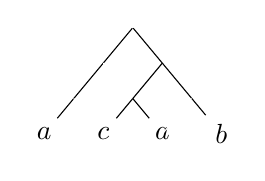
\begin{tikzpicture}[xscale=0.5, yscale=0.3]
      \node[minimum size=0pt, inner sep=0pt] {}
      child {
        child {
          child {node {$a$}}
          child[color=white] {}
        }
        child[color=white] {}
      }
      child {
        child {
          child {node {$c$}}
          child {node {$a$}}
        }
        child {
          child[color=white] {}
          child {node {$b$}}
        }
      };
    \end{tikzpicture}
  \end{equation*}
  which corresponds to the parenthesized product $a \cdot ((c \cdot a) \cdot b)$.
  According to the multiplication table, this product equals $a$.
\end{example}

If $(g_0, \dotsc, g_k)$ is a finite sequence of quasigroup elements denoted $\mathbf{g}$ and $P$ is a parenthesization of that sequence, then the \emph{cube of $\mathbf{g}$ with respect to $P$}, denoted $\cube(\mathbf{g}, P)$, is defined
\begin{equation*}
  \cube_P(\mathbf{g}) = \left\{P(g_0, g_1^{\epsilon_1}, \dotsc, g_k^{\epsilon_k}) \, \middle| \, \epsilon_i \in \{0, 1\} \text{ for each } i \right\}.
\end{equation*}
(This is called a ``cube'' because each vertex of the $k$-dimensional hypercube, when interpreted as a binary string $\epsilon_1 \dotsb \epsilon_k$, yields a quasigroup element.)
If $\cube_P(G) = G$, then $g$ is called a \emph{cube generating sequence of size $k + 1$} for the quasigroup $G$.
The \emph{rank of a quasigroup} is the minimum size of a cube generating sequence.
\footnote{
  This is a nonstandard definition of ``rank'' for quasigroups.
  Elsewhere, the rank of a quasigroup is the number of blocks in the partition of the quasigroup into conjugacy classes according to the action of the quasigroup on itself.
}

\todo{Example of a cube generating sequence for a quasigroup.}

If the quasigroup $G$ is a group, then the operation is associative, so the parenthesization is superfluous (that is, for any parenthesization $P$ and any sequence $(g_0, \dotsc, g_k)$, we have $P(g_0, \dotsc, g_k) = g_0 \cdot \dotsb \cdot g_k$).
If $S$ is a subset of group elements, the \emph{subgroup generated by $S$}, denoted $\gen{S}$, is the closure of $S$ under the group operation.
If $\gen{S} = G$, then $S$ is called a \emph{generating set for $G$}.
The \emph{rank of a group} is the minimum cardinality of a generating set.
Contrast the rank of a group with the rank of a quasigroup: the former is the size of a set, the latter the size of a sequence.

\todo{Example of a generating set for a group.}

\section{Efficient computation of cube membership}

\todo{Introduction and summary paragraph here.}

The \textsc{Cube Membership} problem is defined as follows.
The inputs are a quasigroup $G$ given as a multiplication table, a quasigroup element $h$, a finite sequence of quasigroup elements $\mathbf{g}$, and a parenthesization $P$ for that sequence.
The problem is to decide whether $h \in \cube_P(\mathbf{g})$.

How does a circuit access a multiplication table for a quasigroup of order $n$?
\footnote{This work avoids representing problems using first-order logic, as in the original definition of $\FOLL$ from \autocite{bklm01}, though the logic definition may provide a more natural representation of this sort of information.}
One way for a circuit to compute the product of two quasigroup elements using the multiplication table is via a multiplexer.
In the multiplexer, each input has $O(\log n)$ bits, since each quasigroup element can be represented with $O(\log n)$ bits and each input is a pair of quasigroup elements.
A multiplexer that selects from $n^2$ inputs, each of length $O(\log n)$, can be implemented by an \emph{unbounded fan-in} circuit of constant depth and size $O(n^2 \log n)$.

\begin{lemma}[{Implicit in \autocite[Theorem~3.4]{ctw13}}]\label{lem:cubemem}
  \textsc{Cube Membership} is decidable by an $\L$-uniform family of unbounded fan-in circuits with size $O(2^k k n^2 \log n)$ and depth $O(d)$, where $n$ is the order of the quasigroup, $k$ is the size of the generating sequence, and $d$ is the depth of the parenthesization.

  In particular, if $k$ is in $O(\log n)$ and $d$ is in $O(\log \log n)$, then the circuit is of size polynomial in $n$ and of depth $O(\log \log n)$.
\end{lemma}
\begin{proof}
  The input to the circuit is the multiplication table for a quasigroup, a quasigroup element $h$, a generating sequence $\mathbf{g}$, and a parenthesization $P$.
  Suppose $\mathbf{g} = (g_0, \dotsc, g_k)$ for some positive integer $k$.
  Since the circuit needs to determine if $h$ is in $\cube_P(\mathbf{g})$, the circuit accepts if and only if there is some sequence of bits $(\epsilon_1, \dotsc, \epsilon_k)$ such that $h = P(g_0, g_1^{\epsilon_1}, \dotsc, g_k^{\epsilon_k})$.
  Thus the circuit consists of $2^k$ subcircuits joined to a single \textsc{or} gate, each subcircuit deciding whether one of the $2^k$ possible $k$-bit sequences $(\epsilon_1, \dotsc, \epsilon_k)$ produces $h$ under the given parenthesization.

  The subcircuit corresponding to binary sequence $(\epsilon_1, \dotsc, \epsilon_k)$ computes the parenthesized product $P(g_0, g_1^{\epsilon_1}, \dotsc, g_k^{\epsilon_k})$.
  Computing the product of two quasigroup elements can be implemented in $O(n^2 \log n)$ size and $O(1)$ depth, as described in the paragraph preceding this lemma.
  Computing the parenthesized product therefore can be implemented in $O(k n^2 \log n)$ size and $O(d)$ depth, where $d$ is the depth of the parenthesization.
  Comparing the element produced this way to the element $h$ can be done with a constant depth, $O(\log n)$ size equality comparison circuit.

  We conclude that the overall size of the circuit is $O(2^k k n^2 \log n)$ and the overall depth of the circuit is $O(d)$.
\end{proof}

The \textsc{Subgroup Membership} problem is defined as follows.
The inputs are a group $G$ given as a multiplication table, a group element $h$ and a finite set $S$ of group elements.
The problem is to decide whether $h \in \gen{S}$.

\begin{lemma}\label{lem:subgroupmem}
  \textsc{Subgroup Membership} is in $\L$.
\end{lemma}
\begin{proof}
  The problem is in $\SL$ \autocite[Section~3]{bm89}, and $\SL = \L$ \cite{reingold08}.
\end{proof}

\section{Efficient computation of quasigroup rank}

\todo{foreword and summary here}

The \textsc{Quasigroup Rank} problem is defined as follows.
Given the multiplication table of a quasigroup and an integer $k$ in binary, decide whether the rank of the quasigroup is $k$ or less.
The \textsc{Group Rank} problem is defined similarly.

The \textsc{Quasigroup Isomorphism} problem is the problem of determining whether there is a bijection between two quasigroups (again, given as multiplication tables) that preserves the quasigroup operation.
This problem is in $\bFOLL$ \autocite[Theorem~3.4]{ctw13}.
Implicit in that algorithm is a $\bFOLL$ algorithm for \textsc{Quasigroup Rank}.

\begin{theorem}[{Implicit in \autocite[Theorem~3.4]{ctw13}}]
  \textsc{Quasigroup Rank} is in $\bFOLL$.
\end{theorem}
\begin{proof}
  By \autocite[Theorem~3.3]{ctw13}, each finite quasigroup with $n$ elements has a generating sequence of size $O(\log n)$ with a parenthesization of depth $O(\log \log n)$.
  The $\bFOLL$ algorithm works as follows on input quasigroup $G$ with $n$ elements (given as a multiplication table) and integer $k$, guaranteed to be in $O(\log n)$.
  \begin{enumerate}
  \item Nondeterministically choose a sequence $\mathbf{g}$ of $k + 1$ quasigroup elements and a parenthesization $P$ of depth $O(\log k)$.
  \item Accept if and only if $h \in \cube_P(\mathbf{g})$ for each $h \in G$.
  \end{enumerate}
  Since each quasigroup element can be represented using $O(\log n)$ bits, and since $k$ is in $O(\log n)$, this algorithm uses $O(\log^2 n)$ bits of nondeterminism to guess the generating sequence and parenthesization in the first step.
  By \autoref{lem:cubemem}, checking membership in $\cube_P(\mathbf{g})$ for each element (in parallel) can be implemented by an unbounded fan-in circuit of size polynomial in $n$ and depth $O(\log \log n)$.
  The correctness of this circuit follows from the correctness of the cube membership circuit.
  We conclude that \textsc{Quasigroup Rank} is in $\bFOLL$.
\end{proof}

This theorem gives an immediate improvement over the previous best upper bound for \textsc{Group Rank}, which was $\L^2$ \cite{lsz77} (see \cite[Proposition~3]{at06} for a brief description of the algorithm).
%$\L^2$ is the class of languages decidable by a deterministic Turing machine using $O(\log^2 n)$ space.

\begin{corollary}\label{cor:grouprank}
  \textsc{Group Rank} is in $\bFOLL \cap \bL$.
\end{corollary}

\autoref{fig:inclusions} shows the chain of inclusions that demonstrates how great an improvement this is.
This also immediately improves the result of \cite[Theorem~7]{at06}, which shows \textsc{Nilpotent Group Rank} is in \P, since
\begin{equation*}
  (\bFOLL \cap \bL) \subseteq \NL \subseteq \P.
\end{equation*}
However, the relationship between \FOLL{} and \L{} remains unknown (the best inclusion known is the uninteresting inclusion $\FOLL \subseteq \AC^1$), so the relationship between $\bFOLL$ and $\bL$ is unknown as well.

\begin{figure}
  \caption{\label{fig:inclusions}$\bFOLL \cap \bL$ is much smaller than both $\L^2$ and \P.}
  \begin{center}
    \begin{tikzpicture}
      \node at (2, 4) (h) {$\P$};
      \node at (0, 6) (g) {$\L^2$};
      \node at (0, 5) (f) {$\bNC^2$};
      \node at (0, 4) (e) {$\bAC^1$};
      \node at (1, 3) (d) {$\AC^1$};
      \node at (1, 2) (c) {$\NL$};
      \node at (1, 1) (b) {$\bL$};
      \node at (-1, 2) (x) {$\bFOLL$};
      \node at (0, 0) (a) {$\bFOLL \cap \bL$};
      \draw (a) to (b);
      \draw (b) to (c);
      \draw (c) to (d);
      \draw (d) to (e);
      \draw (e) to (f);
      \draw (f) to (g);
      \draw (a) to (x);
      \draw (x) to (e);
      \draw (d) to (h);
    \end{tikzpicture}
  \end{center}
\end{figure}

%% This is an improvement because
%% \begin{align*}
%%   (\bFOLL \cap \bL) & \subseteq \bL \subseteq \NL \subseteq \AC^1 \subseteq \bAC^1, \\ %\subseteq \bNC^2 \subseteq \L^2,
%%   (\bFOLL \cap \bL) & \subseteq \bFOLL \subseteq \bAC^1, %\subseteq \bNC^2 \subseteq \L^2.
%% \end{align*}
%% and
%% $$
%% \bAC^1 \subseteq \bNC^2 \subseteq \L^2.
%% $$
%% (In the last inclusion we use the fact that $\bNC^2 \subseteq \L^2$ \cite[Lemma~3.1]{wolf94}.)

The complexity of \textsc{Group Rank} contrasts with the related problem of computing the rank of a subgroup of a free group.
That problem is \P-complete, so is not even in \NC{} unless $\NC = \P$ \autocite[Theorem~4.9]{am84} (see also \autocite[Problem~A.8.11]{ghr95}).

\begin{proof}[Proof of \autoref{cor:grouprank}]
  Since a group is a quasigroup, \textsc{Group Rank} is in $\bFOLL$ because \textsc{Quasigroup Rank} is.
  Thus, it suffices to show a $\bL$ algorithm for \textsc{Group Rank}.
  As in the previous theorem, a group has a generating set of size $O(\log n)$.
  The algorithm proceeds as follows on input group $G$ of order $n$ given as a multiplication table and integer $k$ guaranteed to be in $O(\log n)$.
  \begin{enumerate}
  \item Nondeterministically choose a set $S$ of $k$ group elements.
  \item Accept if and only if $h \in \gen{S}$ for each $h \in G$.
  \end{enumerate}
  This algorithm uses $O(\log^2 n)$ bits of nondeterminism in step 1, since each group element can be represented using $O(\log n)$ bits, and $k$ is in $O(\log n)$.
  In step 2, enumerating each $h$ requires only $O(\log n)$ bits of space, since the space can be reused after each iteration.
  By \autoref{lem:subgroupmem}, checking membership in $\gen{S}$ can be decided by a Turing machine using $O(\log n)$ space.
  The correctness of this algorithm follows from the correctness of the subgroup membership algorithm.
  Therefore this is a correct algorithm for deciding \textsc{Group Rank} in $\bL$.
\end{proof}

Although the precise relationship between $\FOLL$ and $\L$ is unknown, $\FOLL$ does not contain any class containing the \textsc{Parity} problem.
Since \textsc{Parity} is in $\L$, we know $\FOLL$ does not contain $\L$.
Stated in a slightly more general way, $\FOLL$ cannot be hard under $\AC^0$ many-one reductions for any complexity class that contains \textsc{Parity} \cite[Proposition~2.1]{bklm01}.
This is true even when the circuit is augmented with a polylogarithmic number of nondeterministic gates \cite[Section~4]{ctw13}.
This gives an immediate improvement to the upper bound of the \textsc{Quasigroup Rank} problem.

\begin{theorem}
  \textsc{Quasigroup Rank} is not hard under $\AC^0$ many-one reductions for any complexity class containing \textsc{Parity}.
\end{theorem}

Specifically, \textsc{Quasigroup Rank} is not hard for any of the classes in the inclusion chain
\begin{equation*}
  \ACC^0 \subseteq \TC^0 \subseteq \NC^1 \subseteq \L \subseteq \NL \subseteq (\LOGCFL \cup \DET).
\end{equation*}

\printbibliography

\end{document}
